\chapter{Pengenalan LLM dalam Dunia Pendidikan}

\section{Apa itu Large Language Model (LLM)?}

Large Language Model (LLM) adalah jenis sistem kecerdasan buatan (AI) yang dirancang untuk memahami dan menghasilkan bahasa alami layaknya manusia. Model ini dilatih menggunakan kumpulan data teks dalam jumlah besar seperti buku, artikel, situs web, dan sumber lainnya untuk mempelajari pola, struktur, serta makna bahasa. Setelah melalui proses pelatihan, LLM mampu memberikan respons yang koheren dan relevan secara konteks terhadap masukan teks, sering kali menyerupai percakapan manusia.

LLM memproses masukan teks dengan mengubahnya menjadi \textbf{token}, yaitu potongan-potongan kecil dari teks seperti kata, suku kata, atau bahkan huruf tergantung konteksnya. Misalnya, kalimat "Saya makan nasi" akan dipecah menjadi token-token seperti "Saya", "makan", dan "nasi". Token inilah yang menjadi dasar bagi model untuk menganalisis dan memprediksi kelanjutan teks.

Token-token tersebut kemudian dianalisis menggunakan \textbf{jaringan saraf tiruan} (neural networks), yaitu sistem komputasi yang meniru cara kerja otak manusia dalam memproses informasi. Dalam konteks LLM, jaringan ini memiliki banyak lapisan yang bekerja untuk memahami hubungan antar token dan konteks di baliknya. Setiap lapisan bertugas mengenali pola-pola tertentu dalam bahasa, seperti tata bahasa, makna, dan gaya penulisan. Hasil dari proses ini adalah kemampuan model untuk memprediksi token berikutnya yang paling sesuai dalam sebuah kalimat atau paragraf.

Istilah "large" pada LLM merujuk pada jumlah parameter yang sangat besar (sering kali mencapai miliaran) yang dipelajari oleh model selama pelatihan. Parameter-parameter ini adalah angka-angka yang mengatur cara model membuat prediksi dan menyusun kalimat. Semakin banyak parameter, semakin besar pula kemampuan model dalam memahami konteks yang kompleks dan menangani berbagai topik serta tugas dengan baik.

Beberapa LLM yang dikenal luas di antaranya:
\begin{itemize}
	\item \textbf{ChatGPT} oleh OpenAI – umum digunakan untuk percakapan, pendamping belajar, dan bantuan penulisan.
	\item \textbf{Claude} oleh Anthropic – menekankan pada aspek keamanan dan keterjelasan interpretasi.
	\item \textbf{Gemini} oleh Google DeepMind – mengintegrasikan kemampuan LLM dalam produk-produk Google.
\end{itemize}

LLM termasuk dalam keluarga besar kecerdasan buatan generatif (generative AI), yang berfokus pada pembuatan konten, bukan hanya analisis. Dalam konteks pendidikan, hal ini membuka peluang hadirnya alat bantu inovatif yang dapat mendukung guru dalam menyiapkan materi, memberikan umpan balik, dan memenuhi kebutuhan belajar yang beragam.



\section{Bagaimana Cara Kerja LLM secara Sederhana}

Untuk memahami cara kerja Large Language Model (LLM) secara sederhana, perhatikan lima langkah utama yang ditampilkan pada Gambar~\ref{fig:diagram-llm}. Diagram tersebut memperlihatkan alur logis mulai dari data hingga keluaran berupa teks yang dihasilkan oleh model AI.

\tikzstyle{process} = [rectangle, rounded corners, minimum width=2cm, minimum height=1cm, text centered, align=center, draw=black, fill=blue!10,  font=\bfseries ]
\tikzstyle{arrow} = [thick,->,>=stealth]

\begin{figure}
	\centering
	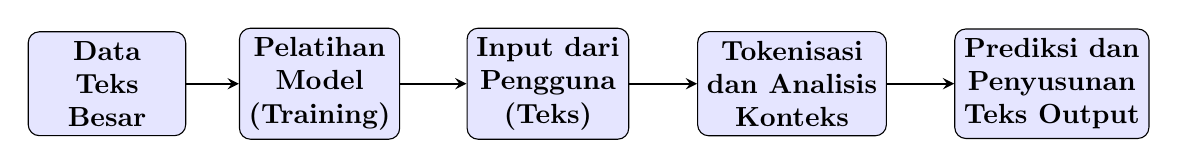
\begin{tikzpicture}[node distance=.1cm, every node/.style={process}]
		\node (data) {Data\\Teks\\Besar};
		\node (training) [right of=data, xshift=2.6cm] {Pelatihan\\Model\\(Training)};
		\node (input) [right of=training, xshift=2.8cm] {Input dari\\Pengguna\\(Teks)};
		\node (token) [right of=input, xshift=3cm] {Tokenisasi\\dan Analisis\\Konteks};
		\node (output) [right of=token, xshift=3.2cm] {Prediksi dan\\Penyusunan\\Teks Output};
		
		\draw [arrow] (data) -- (training);
		\draw [arrow] (training) -- (input);
		\draw [arrow] (input) -- (token);
		\draw [arrow] (token) -- (output);
	\end{tikzpicture}
	\caption{Diagram Sederhana Cara Kerja LLM}
	\label{fig:diagram-llm}
\end{figure}

\textbf{1. Data Teks Besar.}  
Semua proses dimulai dari kumpulan data dalam skala besar yang terdiri dari miliaran kata—berasal dari buku, artikel ilmiah, berita, percakapan daring, dan berbagai sumber lain. Data ini digunakan sebagai dasar pembelajaran agar model mengenali struktur dan makna bahasa.

\textbf{2. Pelatihan Model (Training).}  
Model dilatih menggunakan data tersebut untuk memahami bagaimana satu kata mengikuti kata lain. Selama pelatihan, model belajar mengenali pola dalam kalimat dan menyesuaikan parameter internalnya agar mampu memprediksi token berikutnya secara akurat. Misalnya, jika diberi teks: "Air mengalir dari pegunungan ke...", maka model belajar menebak token berikutnya, seperti "sungai".

\textbf{3. Input dari Pengguna (Teks).}  
Setelah model selesai dilatih, ia dapat digunakan oleh pengguna melalui input teks. Input ini bisa berupa pertanyaan, perintah, atau topik tertentu. Misalnya, pengguna bisa menulis: "Tuliskan ringkasan tentang proses fotosintesis."

\textbf{4. Tokenisasi dan Analisis Konteks.}  
Input teks tersebut dipecah menjadi potongan-potongan kecil yang disebut token. Token ini kemudian dianalisis oleh jaringan saraf tiruan untuk memahami makna dan konteksnya. Model mempertimbangkan hubungan antar-token untuk memahami maksud keseluruhan dari teks yang dimasukkan.

\textbf{5. Prediksi dan Penyusunan Teks Output.}  
Berdasarkan pemahaman terhadap konteks, model mulai menyusun jawaban dengan memprediksi token-token berikutnya secara bertahap. Token-token ini disusun menjadi kalimat yang koheren, hingga terbentuklah teks yang utuh dan relevan dengan input yang diberikan.

Proses ini berlangsung dengan sangat cepat—dalam hitungan milidetik—dan memungkinkan pengguna menerima tanggapan seketika yang tampak alami dan masuk akal. Dengan mengenali tahapan-tahapan ini, penggunaan LLM dapat menjadi lebih terarah dan efektif dalam mendukung aktivitas pembelajaran.



\section{Penggunaan LLM di Kelas: Studi Kasus}

Large Language Model (LLM) seperti ChatGPT dapat menjadi asisten cerdas bagi guru dalam berbagai aktivitas pembelajaran. Dalam konteks kelas, LLM dapat digunakan untuk mempercepat persiapan materi, memperkaya pembelajaran, serta memberikan dukungan terhadap kebutuhan belajar yang beragam. Berikut ini adalah beberapa studi kasus penggunaan LLM secara praktis di lingkungan sekolah:

\textbf{1. Membuat Materi Ajar dan Soal.}  
Gunakan LLM untuk menghasilkan rencana pembelajaran, bahan ajar, dan latihan soal sesuai topik tertentu. Misalnya, untuk topik “Perubahan Iklim” dalam mata pelajaran Geografi, cukup berikan perintah seperti: \texttt{“Buat ringkasan materi dan latihan pilihan ganda untuk siswa SMA tentang perubahan iklim”}. Dalam hitungan detik, model akan menyusun konten tersebut lengkap dengan jawaban dan penjelasan.

\textbf{2. Menyederhanakan Konten Kompleks.}  
LLM mampu menyederhanakan bacaan ilmiah atau dokumen teknis menjadi versi yang lebih mudah dipahami. Ini sangat berguna untuk mendukung literasi sains atau saat membahas artikel berita ilmiah. Contohnya, artikel jurnal dapat disederhanakan dengan prompt seperti: \texttt{“Sederhanakan artikel ini untuk siswa kelas 10 dengan penjelasan yang mudah dimengerti”}.

\textbf{3. Memberikan Umpan Balik Otomatis.}  
Dalam tugas esai atau laporan, LLM dapat digunakan untuk memberi komentar konstruktif. Salin jawaban siswa lalu gunakan prompt seperti: \texttt{"Berikan umpan balik yang membangun atas tulisan ini ber\-da\-sar\-kan struktur, isi, dan tata bahasa"}. Ini sangat membantu menghemat waktu, ter\-u\-ta\-ma untuk kelas besar.

\textbf{4. Adaptasi Pembelajaran untuk Kebutuhan Khusus.}  
Gunakan LLM untuk membuat versi alternatif dari materi pembelajaran bagi siswa dengan kebutuhan khusus, seperti hambatan membaca atau siswa ESL (English as a Second Language). Misalnya, gunakan prompt: \texttt{“Buat versi teks ini dengan kalimat lebih pendek dan kosakata yang sederhana”}.

\textbf{5. Simulasi dan Diskusi Kelas.}  
Ciptakan skenario diskusi atau simulasi peran menggunakan LLM. Dalam pelajaran Sejarah, misalnya: \texttt{“Tuliskan percakapan i\-ma\-ji\-na\-tif antara Soekarno dan Mahatma Gandhi tentang kemerdekaan”}. Aktivitas ini dapat memicu diskusi kritis dan memperkaya kreativitas siswa.

Dengan berbagai cara tersebut, LLM menjadi alat bantu yang fleksibel dan adaptif untuk memperkaya pembelajaran. Meski begitu, penggunaannya tetap perlu pengawasan agar hasil yang digunakan tetap relevan, akurat, dan sesuai konteks.


\section{Demonstrasi Langsung}

Untuk memahami bagaimana Large Language Model (LLM) seperti ChatGPT bekerja dan dimanfaatkan dalam pembelajaran, ikuti demonstrasi langsung berikut. Amati bagaimana model merespons berbagai perintah (prompt), dan nilai secara kritis hasil yang diberikan.

\textbf{1. Lihat Alur Interaksi dengan LLM.} Jalankan web browser, lalu buka aplikasi web ChatGPT \url{https://chatgpt.com}. Perhatikan bagaimana antarmuka aplikasi digunakan untuk mengajukan pertanyaan, menyusun prompt yang efektif, dan menerima hasil dalam hitungan detik. Pahami bagaimana struktur prompt memengaruhi jenis jawaban yang dihasilkan.


\textbf{2. Cobalah Beberapa Prompt Berikut.} Berikut beberapa contoh prompt yang dapat dicoba secara langsung:
\begin{itemize}
	\item \texttt{“Buatkan rencana pelajaran selama 1 jam untuk topik fotosintesis ting\-kat SMA.”}
	\item \texttt{“Buat 5 soal pilihan ganda mengenai revolusi industri be\-ser\-ta ja\-wab\-an\-nya\-.”}
	\item \texttt{“Sederhanakan artikel berikut untuk siswa kelas 8.”}
	\item \texttt{“Tuliskan komentar umpan balik untuk esai siswa berikut.”}
\end{itemize}


\textbf{3. Evaluasi Hasil yang Dihasilkan.} Tinjau hasil dari masing-masing prompt. Apakah sesuai dengan konteks pembelajaran? Apakah ada bagian yang perlu diperbaiki atau disesuaikan? Gunakan penilaian profesional untuk memutuskan apakah konten tersebut siap digunakan atau perlu revisi.


\textbf{4. Eksplorasi Mandiri.} Gunakan waktu yang tersedia untuk mencoba membuat prompt sendiri sesuai mata pelajaran atau kebutuhan yang sedang dihadapi. Bandingkan hasil yang diperoleh dengan ekspektasi. Ubah gaya, tingkat kesulitan, atau format untuk melihat variasi respons.


\textbf{5. Simpan dan Dokumentasikan.} Jika menemukan hasil yang berguna, tangkap layar atau salin hasilnya sebagai dokumentasi. Gunakan sebagai referensi untuk eksperimen lanjutan atau bahan pelengkap kegiatan pembelajaran.


Demonstrasi ini dirancang untuk mendorong eksplorasi aktif dan reflektif terhadap potensi LLM, serta membiasakan penggunaan teknologi ini secara efektif, kreatif, dan etis.


\section*{Latihan Praktik: Mengeksplorasi Prompt ChatGPT}
\addcontentsline{toc}{section}{Latihan Praktik: Mengeksplorasi Prompt ChatGPT}
\begin{itemize}
	\item \textbf{Tujuan:} Memahami bagaimana struktur prompt memengaruhi respons AI.
	\item \textbf{Tugas:} Coba prompt berikut di ChatGPT atau LLM lainnya:  
	\begin{quote}
		\texttt{"Buat rencana pembelajaran 30 menit untuk pelajaran biologi SMA tentang fotosintesis."}
	\end{quote}
	\item \textbf{Tantangan:} Ubah prompt tersebut untuk:
	\begin{itemize}
		\item Menargetkan mata pelajaran lain (misalnya, matematika, sastra)
		\item Menyesuaikan tingkat kelas (misalnya, SMP vs. SMA)
		\item Meminta format alternatif (misalnya, kerja kelompok, flipped classroom)
		\item Silahkan bereksperimen dengan berbagai kondisi spesifik.
	\end{itemize}
\end{itemize}
